\documentclass[tikz,border=6pt]{standalone}
\usepackage[T1]{fontenc}
\usepackage[utf8]{inputenc}
\usepackage{pgfplots}
\usepgfplotslibrary{groupplots}
\usetikzlibrary{calc}
\pgfplotsset{compat=1.18}
\begin{document}
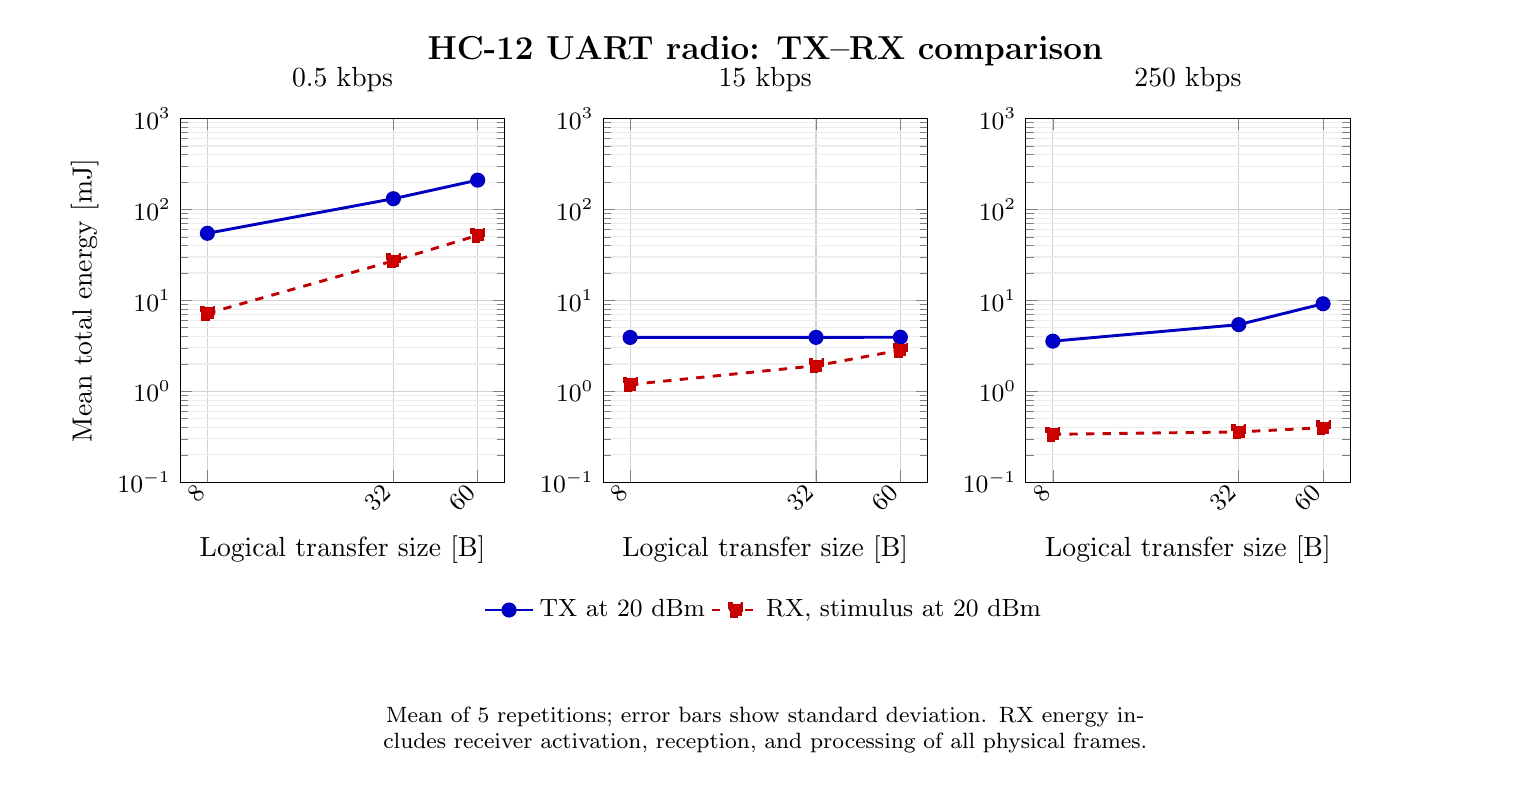
\begin{tikzpicture}
\begin{groupplot}[/pgf/number format/use comma,
  group style={group size=3 by 1, horizontal sep=1.25cm},
  width=5.7cm, height=6.2cm,
  xmode=log, log basis x={2}, ymode=log, log basis y={10},
  ymin=0.1, ymax=1000,
  xtick={8,32,60}, xticklabels={8,32,60},
  x tick label style={rotate=45, anchor=east, font=\small},
  y tick label style={font=\small},
  grid=both, minor grid style={gray!15}, major grid style={gray!35},
  xlabel={Logical transfer size [B]},
  every axis plot/.append style={line width=1.05pt},
  error bars/error bar style={line width=0.35pt},
  legend style={font=\small, draw=none, fill=none, at={(0.5,-0.29)},
    anchor=north, legend columns=-1},
]
\nextgroupplot[title={0.5 kbps}, ylabel={Mean total energy [mJ]}]
\addplot+[color=blue!75!black, solid, mark=*, mark size=2.2pt,
  error bars/.cd, y dir=both, y explicit,
] coordinates {
  (8,54.7319202) +- (0,0.0501987526)
  (32,131.430856) +- (0,5.94934072)
  (60,210.386969) +- (0,11.6108495)
};
\addplot+[color=red!75!black, dashed, mark=square*, mark size=2.2pt,
  error bars/.cd, y dir=both, y explicit,
] coordinates {
  (8,7.20049393) +- (0,0.0042275146)
  (32,27.2146418) +- (0,0.0306695417)
  (60,51.9556272) +- (0,0.0397845648)
};
\nextgroupplot[title={15 kbps}]
\addplot+[color=blue!75!black, solid, mark=*, mark size=2.2pt,
  error bars/.cd, y dir=both, y explicit,
] coordinates {
  (8,3.91501601) +- (0,0.0119927687)
  (32,3.92126592) +- (0,0.00367067511)
  (60,3.93444517) +- (0,0.0207156758)
};
\addlegendentry{TX at 20 dBm}
\addplot+[color=red!75!black, dashed, mark=square*, mark size=2.2pt,
  error bars/.cd, y dir=both, y explicit,
] coordinates {
  (8,1.18750843) +- (0,0.00147193613)
  (32,1.9112527) +- (0,0.0049852535)
  (60,2.83823656) +- (0,0.0118722749)
};
\addlegendentry{RX, stimulus at 20 dBm}
\nextgroupplot[title={250 kbps}]
\addplot+[color=blue!75!black, solid, mark=*, mark size=2.2pt,
  error bars/.cd, y dir=both, y explicit,
] coordinates {
  (8,3.56210357) +- (0,0.0427165399)
  (32,5.41255194) +- (0,0.018580906)
  (60,9.18572541) +- (0,0.0436861039)
};
\addplot+[color=red!75!black, dashed, mark=square*, mark size=2.2pt,
  error bars/.cd, y dir=both, y explicit,
] coordinates {
  (8,0.336648672) +- (0,0.0248390576)
  (32,0.357794074) +- (0,0.0148906677)
  (60,0.397795915) +- (0,0.0149253712)
};
\end{groupplot}
\node[font=\bfseries\large] at ($(group c2r1.north)+(0,0.85cm)$)
  {HC-12 UART radio: TX--RX comparison};
\node[font=\footnotesize, align=center, text width=18.5cm]
  at ($(group c2r1.south)+(0,-3.15cm)$)
  {Mean of 5 repetitions; error bars show standard deviation. RX energy includes receiver activation, reception, and processing of all physical frames.};
\end{tikzpicture}
\end{document}
